%设置整个文档字体大小,纸张
\documentclass[UTF8,a4paper,10pt]{ctexart}

%设置页面格式
\usepackage[left=2.50cm, right=2.50cm, top=2.50cm, bottom=2.50cm]{geometry}


%可以用于禁止浮动体浮动
\usepackage{float}



% \usepackage{titlesec}
% \titleformat{\section}{\raggedright\normalsize\bfseries}{}{-1em}{}
% \titleformat{\subsection}{\raggedright\small\bfseries}{}{-1em}{}

%表格竖线连续化
\usepackage{makecell}
\newcommand\toprule{\Xhline{.08em}}
\newcommand\midrule{\Xhline{.05em}}
\newcommand\bottomrule{\Xhline{.08em}}

%!\I 就可以代替| 来画表格了
\def\I{\vrule width1.2pt}


\usepackage{amsmath,xcolor}
\usepackage{array}
\makeatletter
\renewcommand*\env@matrix[1][*\c@MaxMatrixCols c]{%
 \hskip -\arraycolsep
 \let\@ifnextchar\new@ifnextchar
 \array{#1}}
\makeatother  


%缩进支持
\usepackage{indentfirst}

%可以插入代码
\usepackage{listings}
%语法高亮支持
\usepackage{xcolor}
%代码格式
\definecolor{dkgreen}{rgb}{0,0.6,0}
\definecolor{gray}{rgb}{0.5,0.5,0.5}
\definecolor{mauve}{rgb}{0.58,0,0.82}
\lstset{ %
	%language=Python,	% 编程语言,这里可以不用先设置,用到的时候再设置
	breaklines,	%自动折行
	%extendedchars=false	%解决代码跨页时,章节标题,页眉等汉字不显示的问题
	keepspaces=false,  
	%tabsize=4 	%设置tab空格数
	showspaces=false,  %不显示空格
	showtabs=false,  
	showstringspaces=true, 
	numbers=left, 
	basicstyle=\footnotesize, 
	numberstyle=\tiny, 
	numbersep=5pt, 
	keywordstyle= \color{ blue!70},	%关键字颜色
	commentstyle= \color{red!50!green!50!blue!50},	%注释颜色 
	frame=shadowbox,	 % 边框格式:阴影效果
	rulesepcolor= \color{ red!20!green!20!blue!20} ,
	escapeinside=``,	 % 英文分号中可写入中文
	xleftmargin=2em,xrightmargin=2em, aboveskip=1em,	%设置页边距
	framexleftmargin=2em
}
%设置章节标题左对齐
\CTEXsetup[format={\Large\bfseries}]{section} 
%超链接颜色,会影响文中中引用的字体颜色
\usepackage[colorlinks,linkcolor=black,anchorcolor=blue,citecolor=black]{hyperref}
%自定义页眉、页脚
\usepackage{fancyhdr}  %使用fancyhdr包自定义页眉页脚
\pagestyle{fancy}
%\pagestyle{plain}%没有页眉,页脚放页数
\renewcommand{\headrulewidth}{0.5pt}
\renewcommand{\footrulewidth}{0.4pt}
\lhead{}
\chead{}
\rhead{}
\lfoot{}
\cfoot{\thepage}
\rfoot{}
%可以使用插图图片相关
\usepackage{caption}
\usepackage{graphicx, subfig}
\begin{document}
\captionsetup[figure]{labelfont={bf},name={Fig.},labelsep=period}
%表头部分
\centerline{\LARGE\textbf{Report of Problem Set 2}} 
\vspace{1cm}
\setlength{\parindent}{1em}{\textbf{Name: }}{\textbf{zihaosheng }}

\setlength{\parindent}{1em}{\textbf{Student ID: 000000000000}}\quad\quad\quad\quad\qquad\qquad\qquad\qquad\qquad\qquad\qquad\qquad\qquad\quad {\textbf{2020/05/04}}

\renewcommand\arraystretch{1.5}
\section{Problem Description}
In this practicing, we will implement an image stitcher that uses image warping and homographies to automatically create an image mosaic. We will focus on the case where we have two input images that should form the mosaic, where we warp one image into the plane of the second image and display the combined views. This problem will give some practice manipulating homogeneous coordinates, computing homography matrices, and performing image warps.

The picture provided by the professor are as follows.
\begin{figure}[H]
	\centering
	\begin{minipage}[t]{0,40\textwidth}	
		\centering
		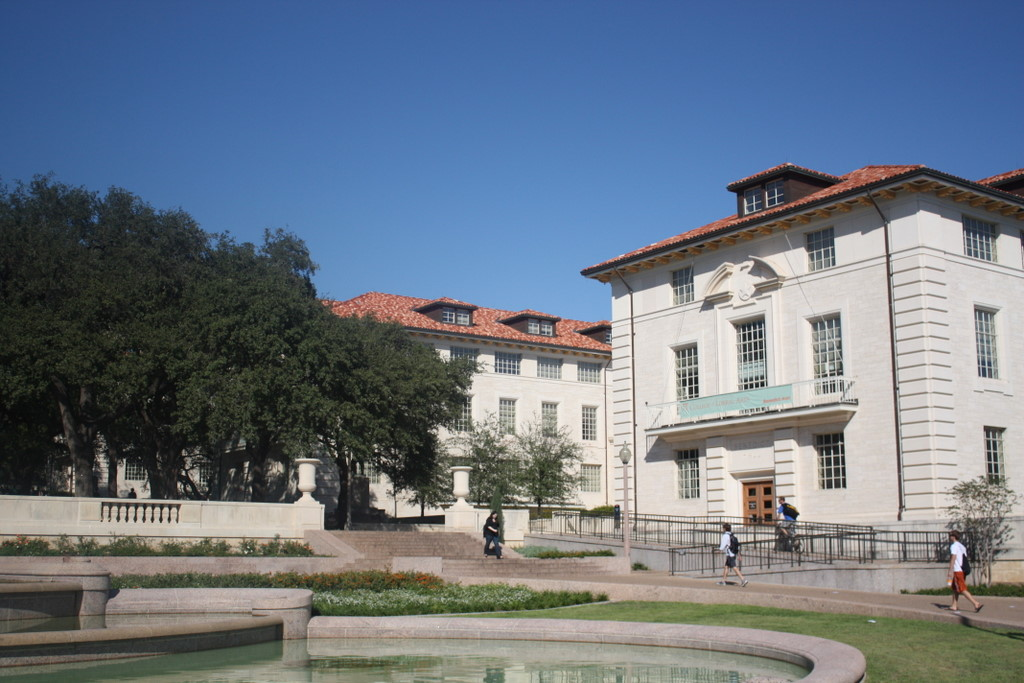
\includegraphics[scale=0.25]{uttower1.JPG} %1.png是图片文件的相对路径
		\caption{Image 1} %caption是图片的标题
		\label{p_ccjg} %此处的label相当于一个图片的专属标志,目的是方便上下文的引用
	\end{minipage}
	\hfil
	\begin{minipage}[t]{0,40\textwidth}	
		\centering
		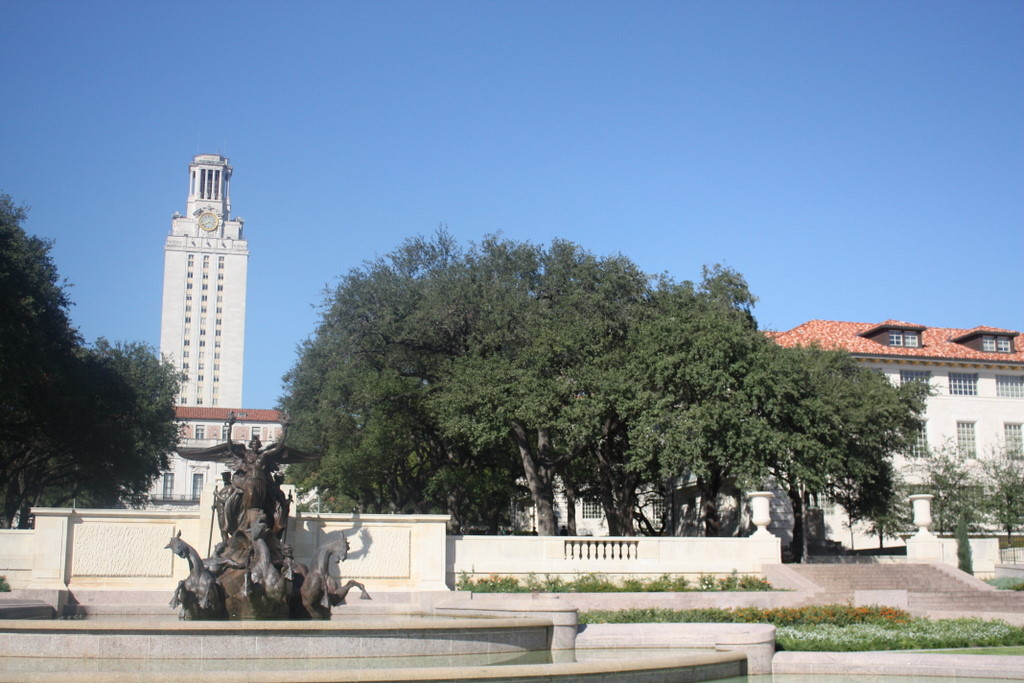
\includegraphics[scale=0.25]{uttower2.JPG} %1.png是图片文件的相对路径
		\caption{Image 2} %caption是图片的标题
		\label{p_AODV} %此处的label相当于一个图片的专属标志,目的是方便上下文的引用
	\end{minipage}
\end{figure}


\section{Implement}
\subsection{Getting correspondences}

First write code to get manually identified corresponding points from two views. The results will be sensitive to the accuracy of the corresponding points; when providing clicks, choose distinctive points in the image that appear in both views.

The points that I chose are as follows. The coordinates of points in Fig. \ref{p1} are (265,229), (477,309), (102,505), (324,530), and coordinates of points in Fig. \ref{p2} are (702,265), (926,329), (563,541), (780,564).
\begin{figure}[H]
	\centering
	\begin{minipage}[t]{0,45\textwidth}	
		\centering
		\includegraphics[scale=0.18]{points1.png} %1.png是图片文件的相对路径
		\caption{Points 1} %caption是图片的标题
		\label{p1} %此处的label相当于一个图片的专属标志,目的是方便上下文的引用
	\end{minipage}
	\hfil
	\begin{minipage}[t]{0,45\textwidth}	
		\centering
		\includegraphics[scale=0.18]{points2.png} %1.png是图片文件的相对路径
		\caption{Points 2} %caption是图片的标题
		\label{p2} %此处的label相当于一个图片的专属标志,目的是方便上下文的引用
	\end{minipage}
\end{figure}

\subsection{Computing the homography parameters}

By homography matrix $H$, we could transform coordinates of points in Fig. \ref{p1} to corresponding points in Fig. \ref{p2}. 
From four pairs of corresponding points, we could list a set of equations with unknowns of $H$.
The homography matrix $H$ that I solved is
$$
H = \begin{bmatrix}
0.735939112 & 0.0127692022 & 453.236174\\ 
-0.133138873 & 0.862093385 & 81.4721190 \\ 
-0.000224348099 & -0.0000928640034 & 1.0 \\ 
\end{bmatrix}
$$

After we solve the homography matrix $H$, we take one point $p_{i}\prime $ in Fig. \ref{p1}, and apply matrix multiplication $Hp_{i}\prime$ to get the coordinate of point $p_{i}$ in Fig. \ref{p2}, where $p_{i}\prime$ and $p_{i}$ are both 3-vectors, and the first two elements of $p_{i}\prime$ are coordinates, and the third is 1. The coordinate of point $p_{i}$ is obtained by dividing the first two elements by the third.
As shown in Fig. \ref{compare}, the corresponding points in two images are connected by lines.
\begin{figure}[htbp]
\centerline{\includegraphics[scale=0.2]{compare.png}}
\caption{Verify the homography matrix.}
\label{compare}
\end{figure}

\subsection{Warping between image planes}

After verifying the homography matrix, we could multiply each coordinate of the Fig. \ref{p1} with the homography matrix to get the warp image. Since the transformed coordinates will typically be sub-pixel values, we could sample the pixel values from nearby pixels. To avoid holes in the output, use an inverse warp. The output image is shown in Fig. \ref{warp}.
\begin{figure}[H]
\centerline{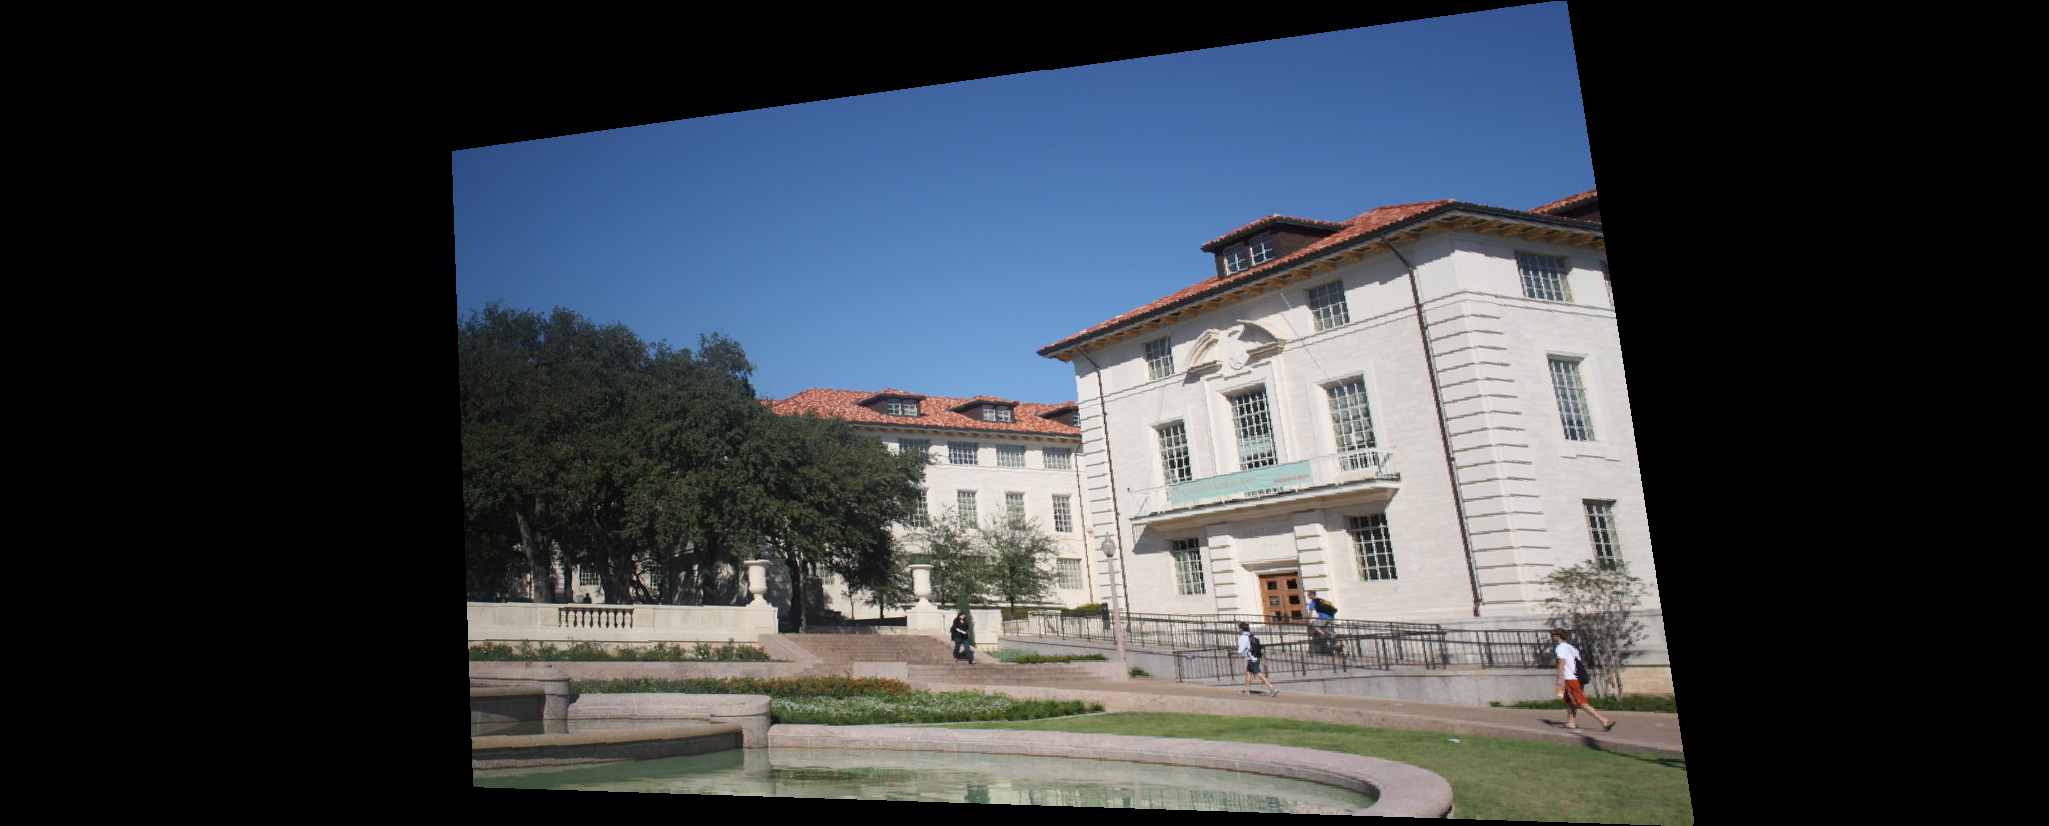
\includegraphics[scale=0.18]{warp.png}}
\caption{A new image that is the warp of the input image using $H$.}
\label{warp}
\end{figure}

\subsection{Create the output mosaic}
Once we have the source image warped into the destination image’s frame of reference, we can create a merged image showing the mosaic, which is shown in Fig. \ref{blend}.
All details are in the file of `main.py'.
\begin{figure}[H]
\centerline{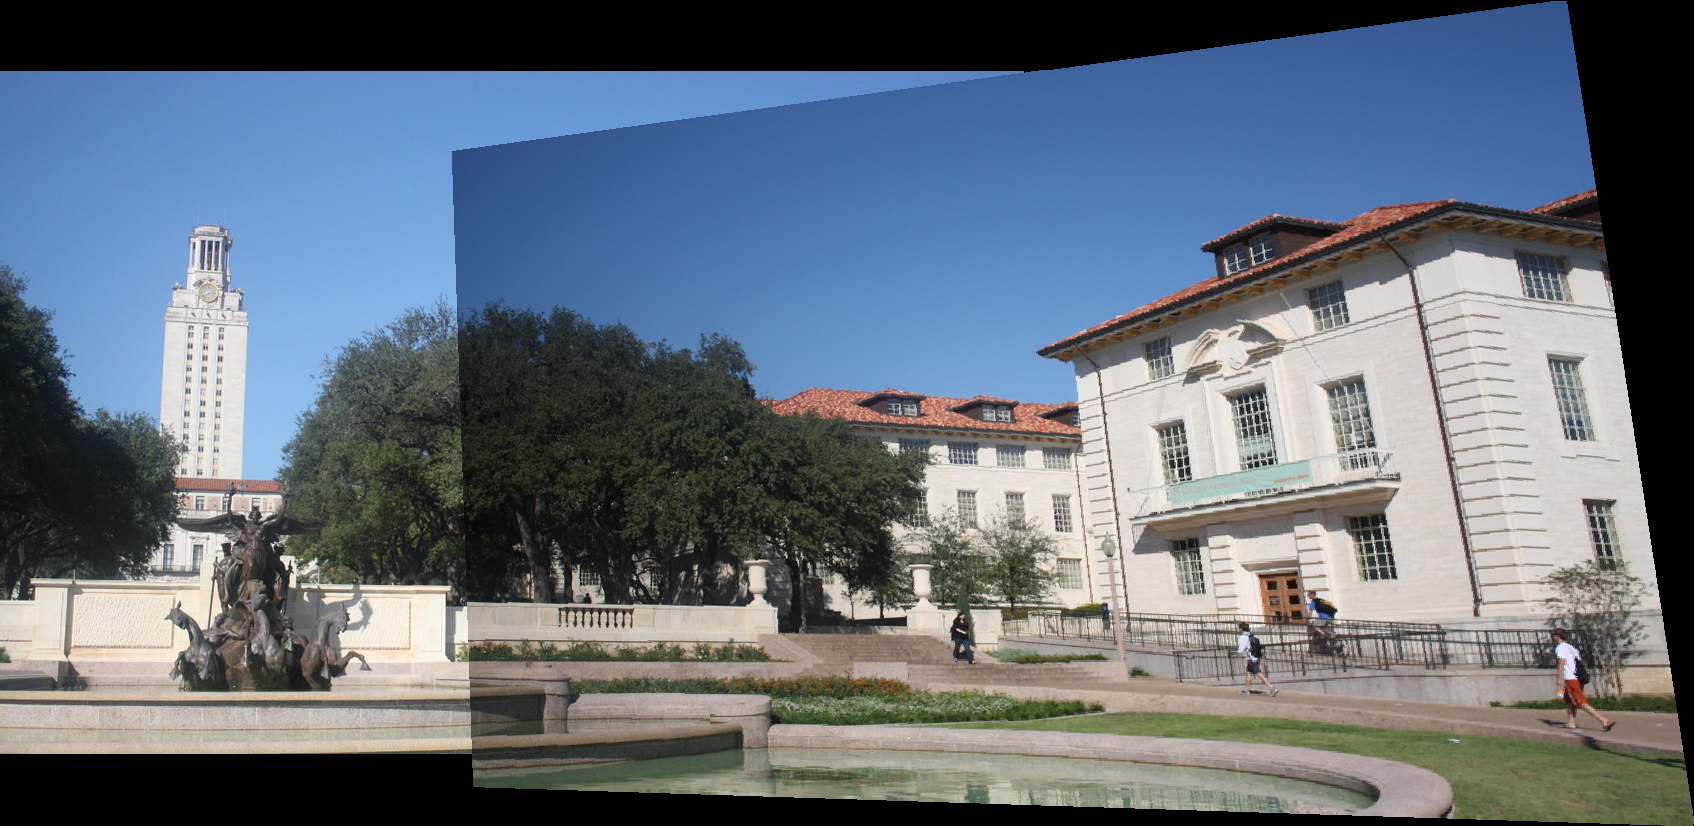
\includegraphics[scale=0.18]{warp_and_blend.png}}
\caption{Blended image.}
\label{blend}
\end{figure}


\section{Another Example}
I show one additional example of a mosaic I create using images that I have taken. The source images are shown as follows.
\begin{figure}[H]
	\centering
	\begin{minipage}[t]{0,40\textwidth}	
		\centering
		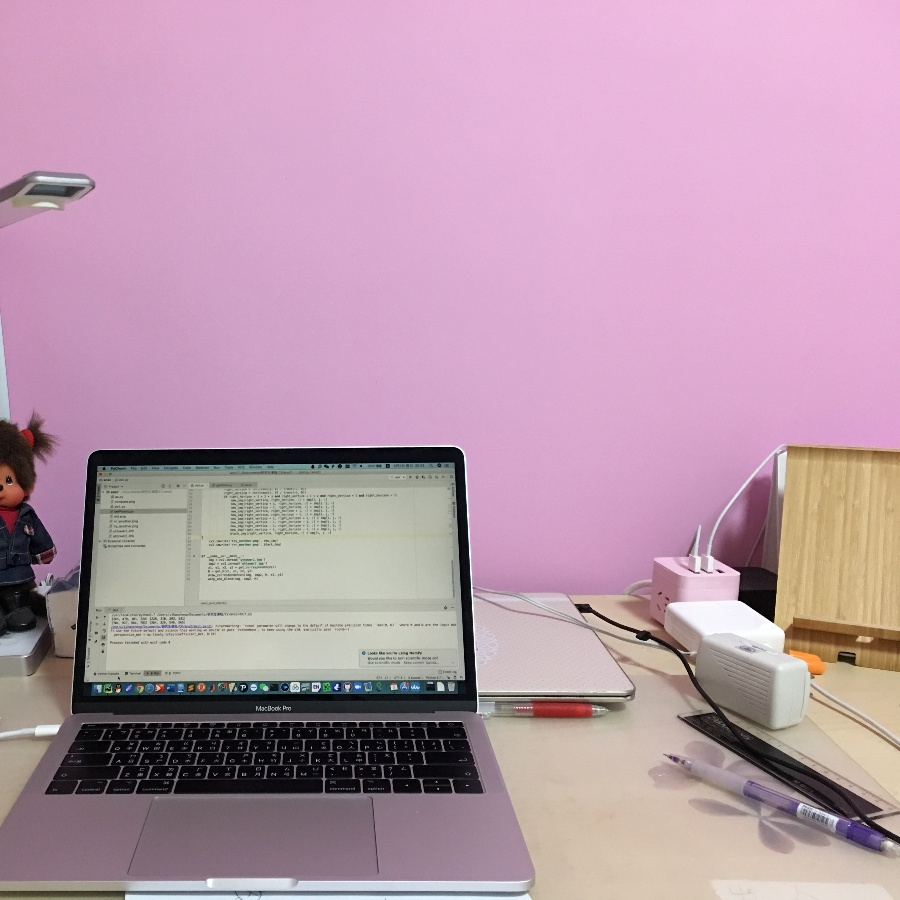
\includegraphics[scale=0.16]{room1.JPG} %1.png是图片文件的相对路径
		\caption{Image 1} %caption是图片的标题
		% \label{} %此处的label相当于一个图片的专属标志,目的是方便上下文的引用
	\end{minipage}
	\hfil
	\begin{minipage}[t]{0,40\textwidth}	
		\centering
		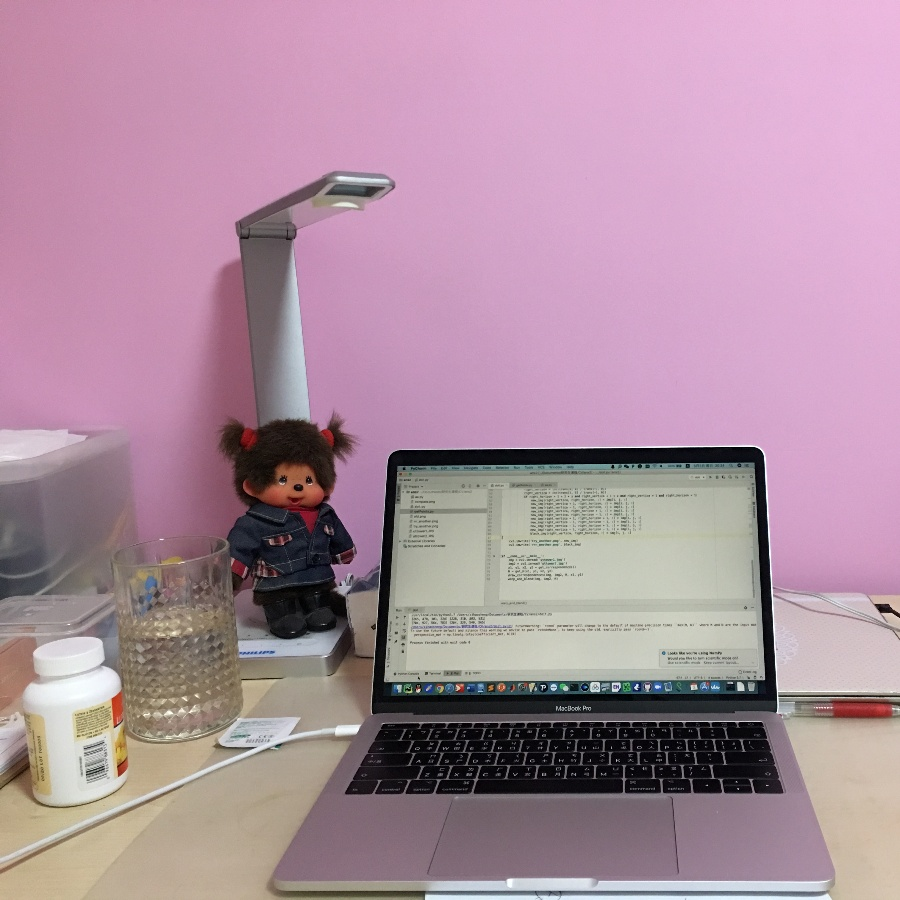
\includegraphics[scale=0.16]{room2.JPG} %1.png是图片文件的相对路径
		\caption{Image 2} %caption是图片的标题
		% \label{p_AODV} %此处的label相当于一个图片的专属标志,目的是方便上下文的引用
	\end{minipage}
\end{figure}

The mosaic that I create is presented in Fig. \ref{key}.
\begin{figure}[H]
\centerline{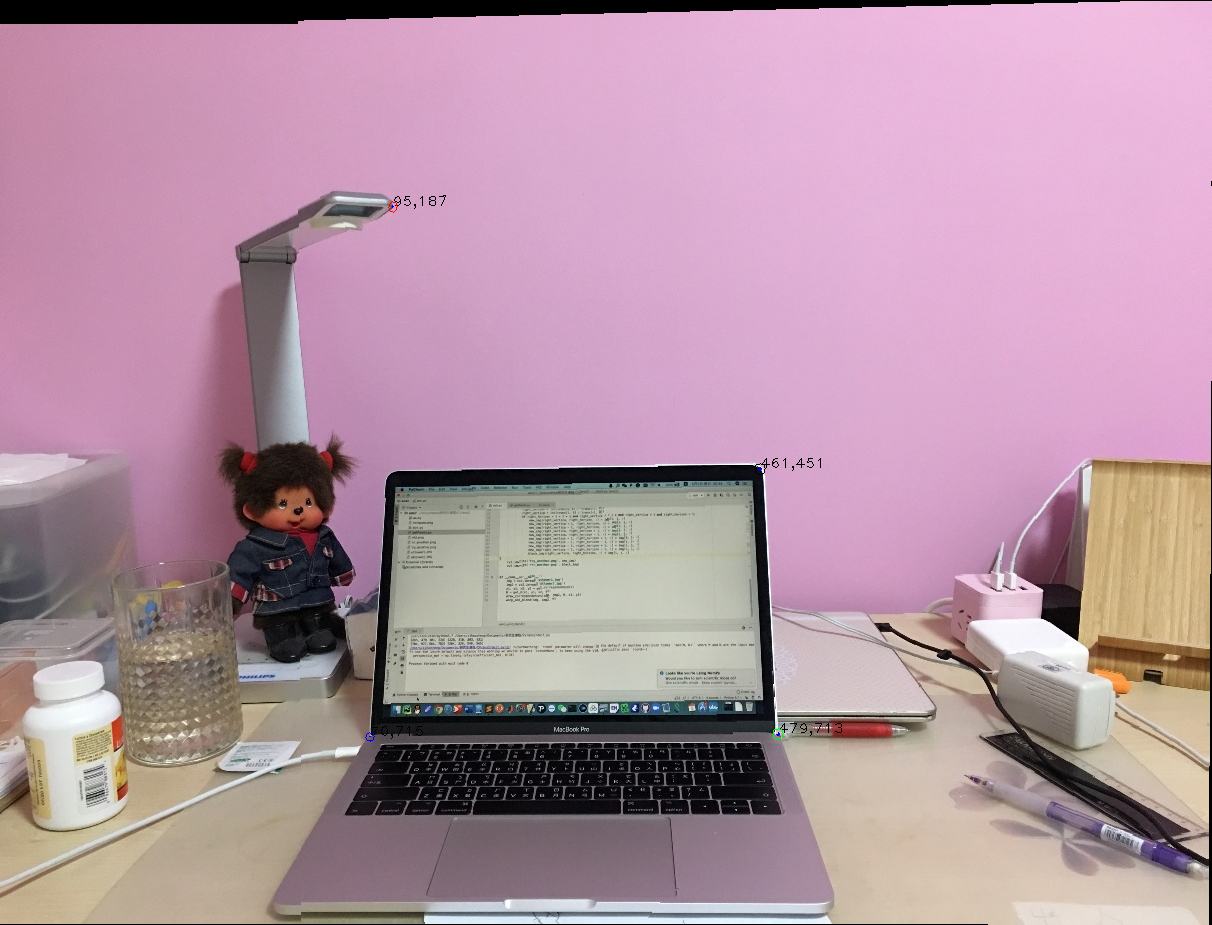
\includegraphics[scale=0.15]{another.png}}
\caption{Blended image.}
\label{key}
\end{figure}

\section{Last Problem}
Fig. \ref{sjtu} is a picture of Shanghai Jiao Tong University, and Fig. \ref{bb} is a billboard to be inserted.
The homography matrix is obtained by transforming the coordinates of the four corners of Fig. \ref{sjtu} to the coordinates of the billboard in Fig. \ref{bb}.
\begin{figure}[H]
	\centering
	\begin{minipage}[t]{0,40\textwidth}	
		\centering
		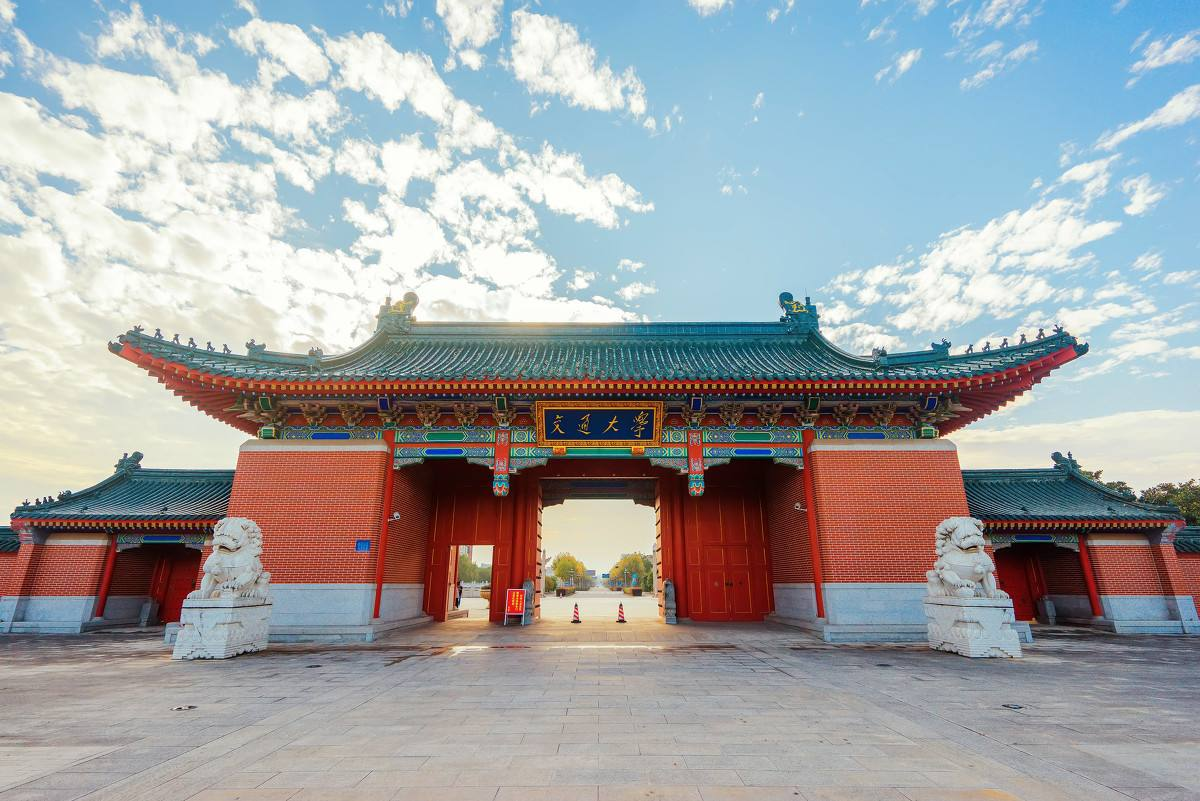
\includegraphics[scale=0.43]{sjtu.JPG} %1.png是图片文件的相对路径
		\caption{SJTU} %caption是图片的标题
		\label{sjtu} %此处的label相当于一个图片的专属标志,目的是方便上下文的引用
	\end{minipage}
	\hfil
	\begin{minipage}[t]{0,40\textwidth}	
		\centering
		
\includegraphics[scale=0.9]{billboard.JPG} %1.png是图片文件的相对路径
		\caption{Billboard} %caption是图片的标题
		\label{bb} %此处的label相当于一个图片的专属标志,目的是方便上下文的引用
	\end{minipage}
\end{figure}

The mosaic that I create is presented in Fig. \ref{key}, and the details are in the file of `insert.py'.
\begin{figure}[H]
\centerline{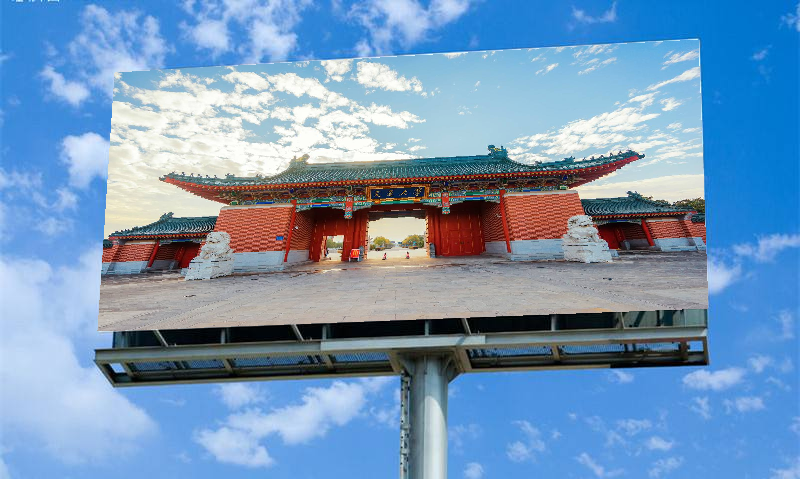
\includegraphics[scale=0.3]{sjtu_on_billboard.png}}
\caption{Mosaic image.}
\label{key}
\end{figure}



% \section{代码}
% \lstset{language=C}
% \begin{lstlisting}[title=PCAdemo.m]
% import cv2
% import numpy as np

% def cross_correlation_2d(img, kernel):# 互相关
%     img_array = np.array(img)  # 把图像转换为数字
%     r= img_array.shape[0]
%     c = img_array.shape[1]  # 图像的列
%     h = img_array.shape[2]  # 图像的高度
%     r2 = kernel.shape[0]  # 核的行
%     c2 = kernel.shape[1]  # 核的列
%     new1 = np.zeros((r, (int)(c2 / 2)), np.int)  #获得一个新的空白矩阵
%     new2= np.zeros(((int)(r2/ 2), c + new1.shape[1] * 2), np.int)
%     conv = np.zeros((r, c, h))
%     for i in range(3):#对矩阵进行一个互相关运算
%         temp_img_array = np.hstack([new1, np.hstack([img_array[:, :, i], new1])]) #对函数增加一个维度
%         new_img_array = np.vstack([new2, np.vstack([temp_img_array, new2])])
%         for j in range(r):
%             for k in range(c):
%                 conv[j][k][i] = min(max(0,(new_img_array[j:j + r2, k:k + c2]* kernel).sum()),255)
%     return conv

% \end{lstlisting}
% References 

% $[1]$ Aude Oliva, Antonio Torralba, and Philippe G Schyns. Hybrid images. ACM Transactions on Graphics (TOG), 2006. http://cvcl.mit.edu/publications/OlivaTorralb_ Hybrid_Siggraph06.pdf.

% $[2]$ Eero Simoncelli. matlabPyrTools. http://www.cns.nyu.edu/~eero/software.php.
\end{document}
%%%%%%%%%%%%%%%%%%%%%%%%%%%%%%%%%%%%%%
%%%%%%%%%%%%
%%%%%%%%%%%%双并列图片示例
%%%%%%%%%%%%
%%%%%%%%%%%%%%%%%%%%%%%%%%%%%%%%%%%%%%
%\begin{figure}[H]
%	\centering
%	\begin{minipage}[t]{0,40\textwidth}	
%		\centering
%		\includegraphics[scale=0.5]{ccjg.pdf} %1.png是图片文件的相对路径
%		\caption{IEEE 802.11层次结构} %caption是图片的标题
%		\label{p_ccjg} %此处的label相当于一个图片的专属标志,目的是方便上下文的引用
%	\end{minipage}
%	\hfil
%	\begin{minipage}[t]{0,50\textwidth}	
%		\centering
%		\includegraphics[scale=1]{AODV.pdf} %1.png是图片文件的相对路径
%		\caption{AODV示意图} %caption是图片的标题
%		\label{p_AODV} %此处的label相当于一个图片的专属标志,目的是方便上下文的引用
%	\end{minipage}
%\end{figure}
%%%%%%%%%%%%%%%%%%%%%%%%%%%%%%%%%%%%%%
%%%%%%%%%%%%
%%%%%%%%%%%%表格示例
%%%%%%%%%%%%
%%%%%%%%%%%%%%%%%%%%%%%%%%%%%%%%%%%%%%
%\begin{table}[H]
%	\centering
%	\caption{802.11a/b/g物理层,MAC层参数}
%	\begin{tabular}{ccccc}
%		\toprule
%		&  参数  & 802.11a & 802.11b & 802.11g \\
%		\midrule
%		\multirow{4}[7]{*}{物理层} & 频带/Hz(freq\_) & $5*10^9$ & $2.4*10^9$ & $2.4*10^9$ \\
%		\cmidrule{3-5}       & 通信感知范围\cite{bib13}(CSThresh\_) & $3.17291*10^9$ & $2.79*10^9$ & $2.79*10^9$ \\
%		\cmidrule{3-5}       & 可通信范围\cite{bib13}(RXThresh\_) & $6.5556*10^{10}$ & $5.76*10^9$ & $5.76*10^9$ \\
%		\cmidrule{3-5}       & 传输功率/W(Pt\_) & 0.281838 & 0.281838 & 0.281838 \\
%		\midrule
%		\multirow{9}[17]{*}{MAC层} & 竞争窗口最小值\cite{bib12}/s(CWMin) & 15 & 31 & 15 \\
%		\cmidrule{3-5}       & 竞争窗口最大值\cite{bib12}/s(CWMax) & 1023 & 1023 & 1023 \\
%		\cmidrule{3-5}       & 时隙\cite{bib11}/s(SlotTime\_) & 0.00005 & 0.00002 & 0.000009s \\
%		\cmidrule{3-5}       & SIFS\cite{bib14}\cite{bib11}/s(SIFS\_) & 0.000016 & 0.00001 & 0.000016s \\
%		\cmidrule{3-5}       & 前导码长度\cite{bib14}(PreambleLength) & 96 & 144 & 120 \\
%		\cmidrule{3-5}       & PLCP头部长度\cite{bib14}PLCPHeaderLength\_) & 24 & 48 & 24 \\
%		\cmidrule{3-5}       & PLCP数据率\cite{bib14}/bps(PLCPDataRate\_) & $6*10^6$ & $1*10^6$ & $6*10^6$ \\
%		\cmidrule{3-5}       & 最高速率\cite{bib14}/bps(dataRate) & $5.4*10^7$ & $1.1*10^7$ & $5.4*10^7$ \\
%		\cmidrule{3-5}       & 最低速率\cite{bib14}/bps(basicRate\_) & $6*10^6$ & $1*10^6$ & $6*10^6$ \\
%		\bottomrule
%	\end{tabular}%
%	\label{t_abgcs}%
%\end{table}%
%%%%%%%%%%%%%%%%%%%%%%%%%%%%%%%%%%%%%%
%%%%%%%%%%%%
%%%%%%%%%%%%插入代码示例
%%%%%%%%%%%%title:代码文件标题
%%%%%%%%%%%%basicstyle:字体大小
%%%%%%%%%%%%language:语言,C++,C,Matlab,Python
%%%%%%%%%%%%%%%%%%%%%%%%%%%%%%%%%%%%%%
%\lstset{language=C++}
%\begin{lstlisting}[title=AODV100.tr,basicstyle=\tiny]
%
%\end{lstlisting}
%%%%%%%%%%%%%%%%%%%%%%%%%%%%%%%%%%%%%%
%%%%%%%%%%%%
%%%%%%%%%%%%对齐公式示例
%%%%%%%%%%%%
%%%%%%%%%%%%%%%%%%%%%%%%%%%%%%%%%%%%%%
%\begin{align}
%	\label{kk}
%	k&=\dfrac{3Z_{11}^{'}}{2(1-l^2_2)^{3/2}}\\
%	\label{hh}
%	h&=\frac{1}{\pi}\left[Z_{00}-\frac{k\pi}{2}+k\arcsin(l_2)+kl_2\sqrt{1-l^2_2} \right]\\
%	\label{ll} l&=\frac{1}{2}\left[\sqrt{\frac{5Z_{40}^{'}+3Z^{'}_{20}}{8Z_{20}}}+\sqrt{\frac{5Z_{11}^{'}+Z^{'}_{11}}{6Z_{11}}}\right]\\
%	\label{pp}
%	\phi&=\arctan\left[\frac{Im[Z_{n1}]}{Re[Z_{n1}]}\right]
%\end{align}
%%%%%%%%%%%%%%%%%%%%%%%%%%%%%%%%%%%%%%
%%%%%%%%%%%%
%%%%%%%%%%%%表格示例2
%%%%%%%%%%%%
%%%%%%%%%%%%%%%%%%%%%%%%%%%%%%%%%%%%%%
%\begin{table}[H]
%	\centering
%	\caption{NVIDIA$^{\textregistered}$ Jetson TK1配置一览}
%	\vspace{0.5cm}
%	\begin{tabular}{l}
%		\Xhline{1.2pt}
%		Tegra K1 SOC \\
%		NVIDIA$^{\textregistered}$ Kepler$^{\textregistered}$ GPU、192 个 CUDA 核心 \\
%		NVIDIA$^{\textregistered}$ 4-Plus-1™ 四核 ARM$^{\textregistered}$ Cortex™-A15 CPU \\
%		2 GB x16 内存、64 位宽度 \\
%		16 GB 4.51 eMMC 内存 \\
%		1 个 USB 3.0 端口、A  \\
%		1 个 USB 2.0 端口、Micro AB\\
%		1 个半迷你 PCIE 插槽\\
%		1 个完整尺寸 SD/MMC 连接器\\
%		1 个 RTL8111GS Realtek 千兆位以太网局域网 \\
%		1 个 SATA 数据端口 \\
%		1 个完整尺寸 HDMI 端口 \\
%		1 个 RS232 串行端口 \\
%		SPI 4 兆字节引导闪存\\
%		1 个带 Mic In 和 Line Out 的 ALC5639 Realtek 音频编解码器\\
%		以下信号可通过扩展端口获得:DP/LVDS, Touch SPI 1x4 + 1x1 CSI-2, GPIOs, UART, HSIC, I$^2$C
%		\\
%		\Xhline{1.2pt}
%	\end{tabular}%
%	\label{aaa}%
%\end{table}%
%%%%%%%%%%%%%%%%%%%%%%%%%%%%%%%%%%%%%%
%%%%%%%%%%%%
%%%%%%%%%%%%双并列表格示例
%%%%%%%%%%%%
%%%%%%%%%%%%%%%%%%%%%%%%%%%%%%%%%%%%%%
%\begin{table}[H]\footnotesize
%	\centering
%	
%	\begin{minipage}[t]{0,47\textwidth}		
%		\caption{上位机配置清单}
%		\vspace{0.5cm}
%		\centering
%		\begin{tabular}{cc}
%			\Xhline{1.2pt}
%			运行环境 & ubuntu14 (基于Cortex$^{\textregistered}$-A15芯片) \\
%			编程语言 & C/C++ \\
%			第三方库及组件 & GTK2.0,OpenCV2.4.10 \\
%			开发环境 & Qt Creator 与 make工程管理器  \\
%			编译工具链 & NVIDIA$^{\textregistered}$-ARM$^{\textregistered}$编译工具链 \\
%			程序结构 & 模块化结构 \\
%			\Xhline{1.2pt}
%		\end{tabular}%
%		
%		\label{pzqd}%
%	\end{minipage}
%	\hfil
%	\hfil
%	\begin{minipage}[t]{0,47\textwidth}	
%		\centering
%		\caption{上位机功能清单}
%		\vspace{0.5cm}	
%		\begin{tabular}{cc}
%			\Xhline{1.2pt}
%			编号  & \multicolumn{1}{c}{功能描述} \\
%			\Xhline{1.2pt}
%			1   & \multicolumn{1}{c}{可打开/关闭摄像头} \\
%			2   & 可通过摄像头捕获图片为目标图片 \\
%			3   & 可从文件系统内选择图片并载入为目标图片 \\
%			4   & 可以检测目标图片中圆形轮廓的半径和圆心 \\
%			5   & 可以检测目标图片中平行直线的间距 \\
%			6   & 检测算法的参数可自由调整 \\
%			\Xhline{1.2pt}
%		\end{tabular}%
%		\label{gn}%
%	\end{minipage}
%\end{table}%